% This is a model template for the solutions in computational science. You can find a very useful documentation for LaTeX in Finnish at ftp://ftp.funet.fi/pub/TeX/CTAN/info/lshort/finnish/ or in English at ftp://ftp.funet.fi/pub/TeX/CTAN/info/lshort/english/. The section List of mathematical symbols in Chapter 3 is especially useful for the typesetting of mathematical formulas.

% Compile the document to PDF by command 'pdflatex model.tex' in the terminal. The command must be run twice for the references in the text to be correct.

\documentclass[a4paper,11pt]{article}
\usepackage[utf8]{inputenc}
% This includes letters such as � and �
\usepackage[T1]{fontenc}
% Use here 'Finnish' for Finnish hyphenation. You may have to compile the code twice after the change. 
\usepackage[english]{babel}
\usepackage{graphicx}
% Some math stuff
\usepackage{amsmath,amsfonts,amssymb,amsbsy,commath,booktabs,hyperref}  
% This is just to include the urls
\usepackage{hyperref,subcaption}
\usepackage[margin=2cm]{geometry}

\setlength{\parindent}{0mm}
\setlength{\parskip}{1.0\baselineskip}

\usepackage{listings}
\usepackage{color}
\usepackage{pdfpages}

\definecolor{dkgreen}{rgb}{0,0.6,0}
\definecolor{gray}{rgb}{0.5,0.5,0.5}
\definecolor{mauve}{rgb}{0.58,0,0.82}

\lstset{frame=tb,
	language=Python,
	aboveskip=3mm,
	belowskip=3mm,
	showstringspaces=false,
	columns=flexible,
	basicstyle={\tiny\ttfamily},
	numbers=none,
	numberstyle=\tiny\color{gray},
	keywordstyle=\color{blue},
	commentstyle=\color{dkgreen},
	stringstyle=\color{mauve},
	breaklines=true,
	breakatwhitespace=true,
	tabsize=4
}

\begin{document}

\title{Becs-114.1100 Computational Science -- exercise round 8} % Replace the exercise round number
\author{Kunal Ghosh, 546247} % Replace with your name and student number
\maketitle
\section{Solution to Question 3}
\subsection{Using Box-Muller algorithm}\label{prob3a}
In this exercise we use the Box-Muller algorithm to generate two gaussing distributed random variables. We generate $10^5$ random number pairs and plot them separately in two histograms shown below.\\
Here we have used the standard python random number generator which uses \textbf{Mersenel Primes} to generate a random number in the range of [0,1]
\begin{figure}[ht]
    \begin{subfigure}{.5 \textwidth}
	\centering
    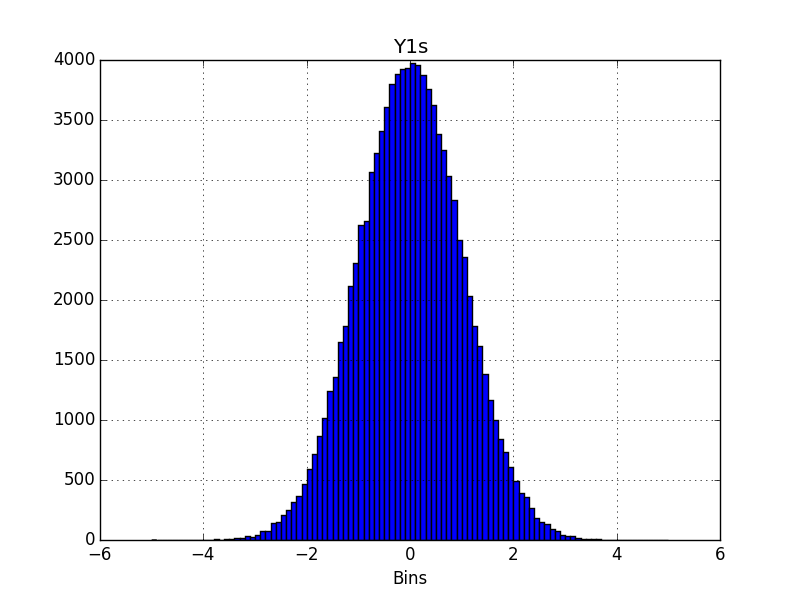
\includegraphics[scale=0.40]{figure3_y1s.png}
    \caption{$Y_1$ as per $\sqrt(-2\log(x1))*\cos(2*\pi*x2)$}
	\label{fig:Y1}
\end{subfigure}
    \begin{subfigure}{.5 \textwidth}
	\centering
    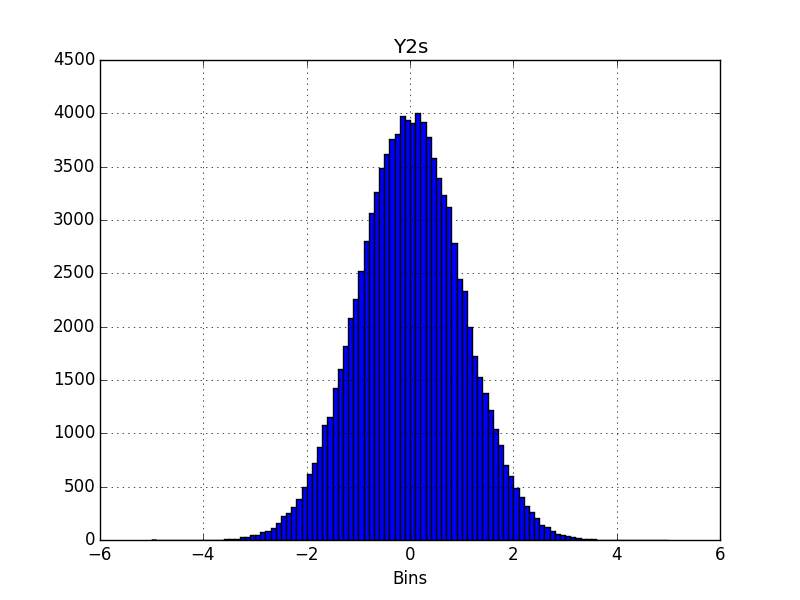
\includegraphics[scale=0.40]{figure3_y2s.png}
    \caption{$Y_1$ as per $\sqrt(-2\log(x1))*\cos(2*\pi*x2)$}
	\label{fig:Y1}
\end{subfigure}
    \caption{This plot shows Y1 and Y2, two random variables generated from two uniformly distributed random variables(x1 and x2) and transformed as showing under the respective graphs.}
\end{figure}

These are two zero mean and unit variance gaussian distributed random numbers.

The corresponding python code can be found at \ref{code:problem3a}
\section{Solution 4a}\label{prob4a}

In this section we compare the 1st, 2nd and 3rd moments of two random number generators. LCG(128, 0, 509) and Mersene Twister. We compare these to the true moments defined by:
\begin{equation}
    \langle x^{k} \rangle = \frac{1}{(k+1)}
\end{equation}
In the above equation k is the moment. i.e. k = 1 gives us the 1st moment, k = 2 gives us the second moment and so on.
We calculate the moments for different random number generators by generating a sequence of $N$ random numbers from the generator and using the formula below. 
\begin{equation}
    \langle x^k \rangle = \frac{1}{N}\sum_{i=1}^{N}x_{i}^{k}
\end{equation}

In this experiment we are trying to see whether the the two random number generators are truly uniform. If they are then their moments must be close to the true moments of the uniform distribution.

\begin{table}[ht]
\centering
\label{1moment}
\begin{tabular}{|c|c|c|c|}
\hline
\textbf{N} & \textbf{LCG(128,0,509)}&\textbf{Mersene Twister}&\textbf{True Moment} \\ \hline
10 & 0.0264746457362 & 0.518080782167 & 0.5 \\
100 & 0.00240679565587 & 0.474926738729 & 0.5 \\
1000 & 0.000238511281212 & 0.494459184012 & 0.5 \\
10000 & 2.38296599591e-05 & 0.493928278685 & 0.5 \\
100000 & 2.38275152683e-06 & 0.500197518937 & 0.5 \\
1000000 & 2.38273008204e-07 & 0.499728476939 & 0.5 \\
10000000 & 2.38272793759e-08 & 0.500054377307 & 0.5 \\
\hline
\end{tabular}
\caption{Values for the 1st Moment}
\end{table}

\begin{table}[ht]
\centering
\label{1moment}
\begin{tabular}{|c|c|c|c|}
\hline
\textbf{N} & \textbf{LCG(128,0,509)}&\textbf{Mersene Twister}&\textbf{True Moment} \\ \hline
10 & 0.00377304392308 & 0.310275753489 & 0.333333333333 \\
100 & 0.000343003993013 & 0.311212396032 & 0.333333333333 \\
1000 & 3.3991386695e-05 & 0.328312667816 & 0.333333333333 \\
10000 & 3.39607913874e-06 & 0.326612059681 & 0.333333333333 \\
100000 & 3.39577348856e-07 & 0.333317261858 & 0.333333333333 \\
1000000 & 3.39574292657e-08 & 0.333169017655 & 0.333333333333 \\
10000000 & 3.3957398704e-09 & 0.3333760948 & 0.333333333333 \\
\hline
\end{tabular}
\caption{Values for the 2nd Moment}
\end{table}

\begin{table}[ht]
\centering
\label{1moment}
\begin{tabular}{|c|c|c|c|}
\hline
\textbf{N} & \textbf{LCG(128,0,509)}&\textbf{Mersene Twister}&\textbf{True Moment} \\ \hline
10 & 0.000640566707312 & 0.199266027703 & 0.25 \\
100 & 5.82333370283e-05 & 0.228229711742 & 0.25 \\
1000 & 5.77087123704e-06 & 0.246069547559 & 0.25 \\
10000 & 5.7656769335e-07 & 0.243561537242 & 0.25 \\
100000 & 5.76515801739e-08 & 0.249764456768 & 0.25 \\
1000000 & 5.76510613091e-09 & 0.249906635608 & 0.25 \\
10000000 & 5.76510094232e-10 & 0.250034371239 & 0.25 \\
\hline
\end{tabular}
\caption{Values for the 3rd Moment}
\end{table}
We can see that in all the 3 cases above, the LCG deviates from each of the moments quite a bit as we take more samples from the random number generator. However, the Mersent Twister stays quite close to the true moment even when we take a lot of samples from the generator which means that the random number it generates are close to uniformly distributed.
% \begin{figure}[ht]
% 	\center
%     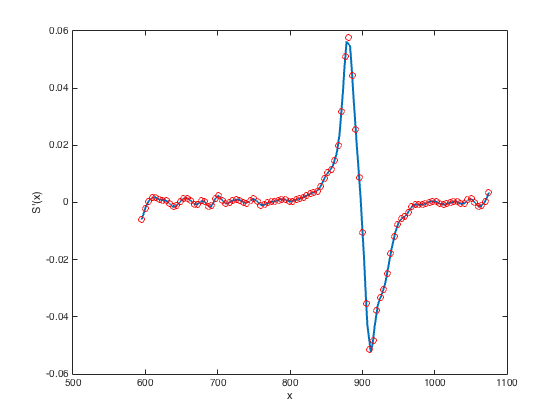
\includegraphics[scale=0.75]{matlabS_dash.png}
%     \caption{Plot showing the first derivative of the natural cubic interpoland S'(X) as calculated using Matlab. Values of $S'(X_i)$ for $X_i$ in the range of (min(knot values), max(knot values)) are shown as red circles.} 
% 	\label{fig:sdash_matlab}
% \end{figure}
% The corresponding plots created by matlab are much more smoother because matlab implements an additional constraint that the third derivatives of the piecewise polynomials are also equal at the second and the last knots. This are apparently called the "Not-A-Knot" end conditions. This is only done when the length of \textbf{t} and \textbf{y} are same.
% 
% Natural splines are a good choice only when the functions have 0 second derivative at the end points. I read it up from here. \url{http://www.mathworks.com/matlabcentral/newsreader/view_thread/172988} would really appreciate some more information about why using the Not-A-Knot condition is better. 
% \\
% The corresponding matlab code can be found at \ref{code:problem2b}

The corresponding python code can be found at \ref{code:problem4a}

\section{Solution 4b}\label{prob4b}
In this solution we are trying to validate the central limit theorem. \textit{An average of measured quantities, taken from the same distribution (which can be any distribution), will asymptotically follow the normal distribution.}
Here we draw random numbers from the uniform distribution and since the generator generates values close to the uniform distribution the mean of the values as we draw more samples tends to the normal distribution.
\begin{figure}[ht]
    \begin{subfigure}{.5 \textwidth}
	\centering
    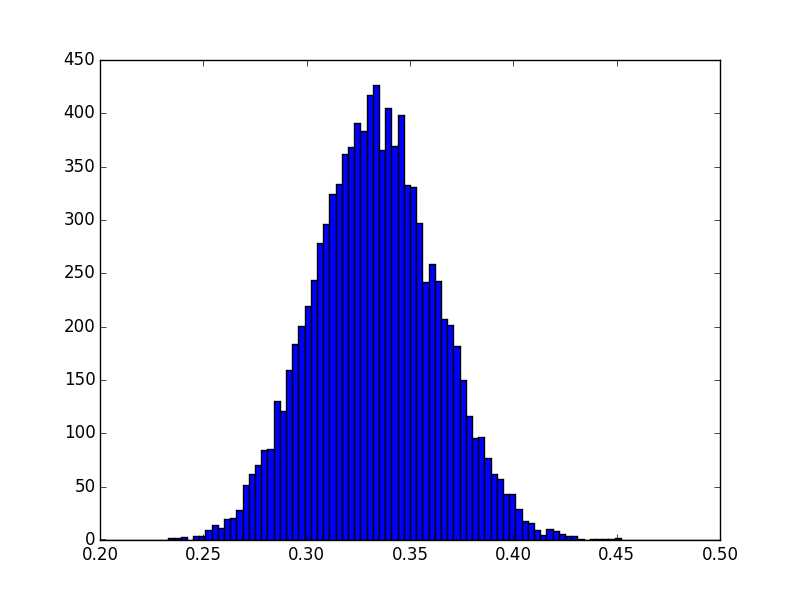
\includegraphics[scale=0.45]{fig4b.png}
    \caption{N = 100, m = 10000}
	\label{fig:clt_10000}
    \end{subfigure}
    \begin{subfigure}{.5 \textwidth}
	\centering
    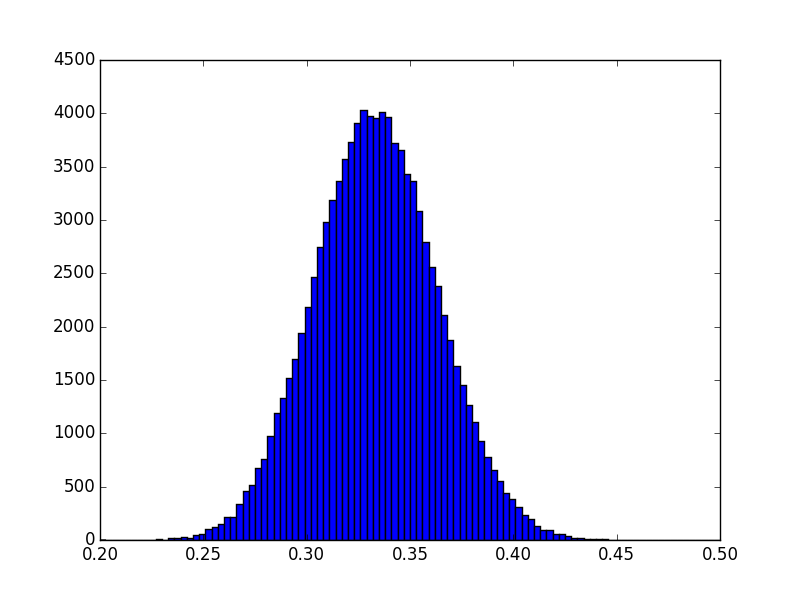
\includegraphics[scale=0.45]{fig4b_100000.png}
    \caption{N = 100, m = 100000}
	\label{fig:clt_100000}
    \end{subfigure}
    \caption{Figure validating the central limit theorem in the figure to the left we have plotted 10000 means of $\langle x^2 \rangle$100 random numbers and can see that the figure is almost like the normal distribution. This is confirmed as the number of means are increased to 100,000 of 100 random numbers and the graph looks very much like the normal distribution. Bins = 100 interval = [0.2,0.5] this interval is chosen because the mean of the values is around 0.33333}
\end{figure}


The corresponding python code can be found at \ref{code:problem4b}
\clearpage
\section{Appendix A}\label{code:problem3a}
Python source code for \ref{prob3a}.
{\footnotesize
\begin{lstlisting}
from __future__ import division
import random
import math
import pylab as pl

pi    = math.pi
log   = math.log
cos   = math.cos
sin   = math.sin
sqrt  = math.sqrt
floor = math.floor

def get_gauss_random():
    x1 = random.random()
    x2 = random.random()

    y1 = sqrt(-2*log(x1))*cos(2*pi*x2)
    y2 = sqrt(-2*log(x1))*sin(2*pi*x2)

    # We don't multiply by sigma
    # implying the value is unit variance

    # Since are random numbers are uniform
    # between 0 and 1, we have zero mean.

    # Hence our distributionis zero mean and 
    # unit variance.
    return y1,y2


def get_bin(yi, ymin, ymax, Nbin):
    val = ((yi - ymin) / (ymax - ymin)) * Nbin
    return floor(val)

if __name__ == '__main__':
    seed = 7777
    random.seed(seed)
    Nbin = 100
    bins = [0] * Nbin
    ymin, ymax = -5, 5
    binVals = []
    ybins = []
    for _ in xrange(100000):
        y = get_gauss_random()
        ybins.append(y)
        #binVals.append(get_bin(yi, ymin, ymax, Nbin))
        # binNum = get_bin(yi, ymin, ymax, Nbin)
        # bins[binNum]+=1
    y1s,y2s = zip(*ybins)
    pl.figure()
    pl.grid()
    pl.hist(y1s,bins=Nbin,range=(ymin,ymax))
    #pl.hist(binVals, bins=Nbin)
    pl.xlabel("Bins")
    pl.title("Y1s")
    pl.savefig("figure3_y1s.png")
    pl.figure()
    pl.grid()
    pl.hist(y2s,bins=Nbin,range=(ymin,ymax))
    #pl.hist(binVals, bins=Nbin)
    pl.xlabel("Bins")
    pl.title("Y2s")
    pl.savefig("figure3_y2s.png")
    pl.show()
\end{lstlisting}
}
\clearpage
\section{Appendix B}\label{code:problem4a}
Python source code \ref{prob4a}.
{\footnotesize
\begin{lstlisting}

from __future__ import division
import random
import math
import pylab as pl

pi    = math.pi
log   = math.log
cos   = math.cos
sin   = math.sin
sqrt  = math.sqrt
floor = math.floor

def lcg(x):
    # Implementing lcg(a,b,m)
    # a = 128 b = 0 m = 509
    a = 128
    b = 0
    m = 509
    randVal = (a*x + b)%m
    return randVal / m # scale the rand num to be in 0,1 range

def get_moment(rand_nums, m):
    return sum([x**m for x in rand_nums])/len(rand_nums)

if __name__ == '__main__':
    seed = 7777
    random.seed(seed)
    randLcg = lcg(seed)   
    lcgs = [randLcg]
    srgl = []
    N = 10**7
    moment = [[],[],[]]
    for _ in xrange(N):
        randLcg = lcg(randLcg)
        lcgs.append(randLcg)
        srgl.append(random.random())
    for m in [1,2,3]:
        trueMoment = 1/(m+1)
        print "M = {}".format(m)
        for N in [10, 100, 1000, 10000, 100000, 1000000, 10000000]:
            lcgMoment = get_moment(lcgs[1:N], m)
            srglMoment = get_moment(srgl[1:N], m)
            moment[m-1].append((lcgMoment, srglMoment, trueMoment))
            print("{} & {} & {} & {} \\\\".format(N,lcgMoment,srglMoment,trueMoment))

 
\end{lstlisting}
}
\section{Appendix C}\label{code:problem4b}
Python source code for \ref{prob4b}.
{\footnotesize
\begin{lstlisting}
from __future__ import division
import random
import math
import pylab as pl

pi    = math.pi
log   = math.log
cos   = math.cos
sin   = math.sin
sqrt  = math.sqrt
floor = math.floor

def get_moment(rand_nums, m):
    return sum([x**m for x in rand_nums])/len(rand_nums)

if __name__ == '__main__':
    seed = 7777
    random.seed(seed)
    N = 100
    m = 10000
    means = []
    for _ in xrange(m):
        temp = 0
        for _ in xrange(N):
            temp += random.random() ** 2
        means.append(temp/N)
    pl.hist(means, bins=100, range=(0.2,0.5))
    pl.savefig("fig4b.png")
    pl.show()
\end{lstlisting}
}
\end{document}

   

